%&encoding=UTF-8 Unicode
\documentclass[12pt,twoside,openany]{fithesis}
\usepackage[resetfonts]{cmap}

% Nastavení fontů.
\usepackage{mathpazo} % Jako základ použít rodinu písem Pazo Math, která 
                      % obsahuje matematické řezy vhodné pro kombinování 
                      % s písmem Palatino.
\usepackage{tgpagella} % Patkové písmo přenastavit na TeX Gyre Pagella (jako 
                       % alternativu písma Palatino).
\usepackage{tgheros} % Bezpatkové písmo přenastavit na TeX Gyre Heros (jako 
                     % alternativu písma Helvetica).
\usepackage{tgcursor} % Strojopisné písmo přenastavit na TeX Gyre Cursor (jako 
                      % alternativu písma Courier).
\pdfpkresolution=1200
\usepackage{cmap}

\usepackage[lmargin=28mm,
	    rmargin=20mm,	
            tmargin=25mm,
            bmargin=30mm,
            includeheadfoot,
            heightrounded,
           ]{geometry}

\usepackage[slovak]{babel}
\AtBeginDocument{\shorthandoff{-"}} % Deaktivuje znaky spojovník (-) a uvozovky 
                              % (") aktivované novou podporou češtiny v balíčku 
                              % "babel", což zabrání problémům se zadáváním 
                              % těchto znaků v parametrech některých maker.
\usepackage[utf8x]{inputenc}
\usepackage[T1]{fontenc}
\usepackage[isu,small,bf,up]{caption2}
\usepackage{pdfpages}


\usepackage{tocloft}




%fasrhdfhdhatdh \usepackage[labelformat=Obrázok]{caption}

\pdfpkresolution1200
\usepackage[protrusion,expansion,step=1]{microtype}
\usepackage[unicode=true,
            plainpages=false,
            pdfpagelabels=true,
            %pdfborder={0 0 0},
            %backref=page,
            pdfpagemode=UseNone,
            pdfstartview={XYZ null null 1},
            pdfpagelayout=OneColumn,
            pdfdisplaydoctitle=true,
            bookmarks=true,
            bookmarksopen=true,
            bookmarksopenlevel=5,
            bookmarksnumbered=true
           ]{hyperref}

\makeatletter
    \let\origsection\section%
    \def\section{%
        \@ifstar%
            {\starsection}%
            {\origsection}}%
    \def\starsection#1{%
        \origsection*{%
            \phantomsection%
            \addcontentsline{toc}{section}{#1}%
            #1}}%
    \let\origsubsection\subsection%
    \def\subsection{%
        \@ifstar%
            {\starsubsection}%
            {\origsubsection}}%
    \def\starsubsection#1{%
        \origsubsection*{%
            \phantomsection%
            \addcontentsline{toc}{subsection}{#1}%
            #1}}%
    \let\origsubsubsection\subsubsection%
    \def\subsubsection{%
        \@ifstar%
            {\starsubsubsection}%
            {\origsubsubsection}}%
    \def\starsubsubsection#1{%
        \origsubsubsection*{%
            \phantomsection%
            \addcontentsline{toc}{subsubsection}{#1}%
            #1}}
\makeatother
\makeatletter
    \def\cleardoublepage{\clearpage\if@twoside \ifodd\c@page\else
        \thispagestyle{empty}
        \hbox{}\newpage\if@twocolumn\hbox{}\newpage\fi\fi\fi}
\makeatother
\mathcode`\,="013B
\def\,{\kern 0.25em}
\newcommand{\tecky}{\kern 0.16667em\dots}
\newcommand{\cssplit}[1]{\discretionary{#1}{#1}{#1}\kern 0pt}
\newcommand{\spj}{\cssplit{-}}
\newcommand{\sls}{\cssplit{/}}
\newcommand{\bsls}{\char`\\}
\let\origurl\url
\def\url#1{\texttt{<\origurl{#1}>}}
\def\email#1{\texttt{<\href{mailto:#1}{#1}>}}
\def\odkaz#1#2{#1 (\url{#2})}
\def\skrytyodkaz#1#2{\href{#2}{#1}}

\widowpenalty10000
\clubpenalty10000
\newcommand{\vhodnyzlom}{\penalty-5000}
\newcommand{\nevhodnyzlom}{\penalty5000}

\setcounter{secnumdepth}{2} %2
\setcounter{tocdepth}{4} %2


%%% Informace o práci:
\thesistitle{\uppercase{NADPIS}	 \\\Large ENGLISH} % Makro umožní vložit název práce, u dvouřádkových 
                   % či víceřádkových názvů se standardně oddělí jednotlivé 
                   % části příkazem \\ s volitelným parametrem meziřádkového 
                   % prokladu.
\thesissubtitle{Bakalárska práca} % Makro umožní vložit název typu práce, např. 
                                  % bakalářská práce, diplomová práce atd.
\thesisstudent{JA} % Makro umožní pomocí svého jediného parametru 
                             % vložit jméno studenta.
\thesiswoman{false} % Makro umožní vložit pohlaví studenta. Možné hodnoty jsou 
                    % true a false.
\thesisfaculty{eco} % Makro umožní stanovit pod jakou fakultou byla práce 
                   % napsána. Podle toho se také vloží patřičné logo a název 
                   % fakulty na titulní stránku. Jsou podporovány fakulty MU fi, 
                   % sci, law, eco, fss, med, ped a phil. Pokud práce není psaná 
                   % pod žádnou z výše uvedených fakult MU, pak je nutné zadat 
                   % i název univerzity \thesisuniversity{}, jméno souboru loga 
                   % fakulty (bez přípony) \thesislogo{} a též do makra 
                   % \thesisyear{} sídlo dané univerzity (pro MU toto není 
                   % třeba).

 \thesisuniversity{Studijní obor: Finance}    
\thesisyear{2013} % Makro umožní vložit rok vypracování práce.
\thesisadvisor{VEDUCI} % Makro umožní vložit jméno vedoucího práce.
\thesislang{sk} % Makro umožní stanovit jazyk, ve kterém je práce napsaná 
                % (v současné době jsou podporovany variany cs, sk, en).
% Makro pro definici klíčových slov práce.
\def\klicovaslova{\hspace{5mm} }%=======KLUCOVE SLOVA
\makeatletter
\hypersetup{%
    pdfauthor={\@thesisstudent},
    pdftitle={\@thesistitle},
    pdfsubject={\@thesissubtitle},
    pdfkeywords={\klicovaslova}
}
\makeatother



\begin{document} % Začátek dokumentu.

\FrontMatter % Pro první strany dokumentu obsahující prohlášení, abstrakt 
             % a klíčová slova se nastaví římské číslování.
\ThesisTitlePage % Vysadí titulní stranu práce. Využije předem zadaných údajů 
                 % názvu práce, jména studenta a roku vypracování\cleardoubl	epage          




     \begin{figure}[h!]	
\begin{tabular}{l l }
\uppercase{Meno a priezvisko autora:~~~~~}	& Bc. Lukáš Ratica	\\ \vspace{1mm}
\uppercase{NÁZOV BAKALÁRSKEJ PRÁCE:}	&	Nemovitost jako investiční instrument\\ \vspace{1mm}
\uppercase{NÁZOV PRÁCE V ANGLIČTINE:}	&	Real property as an investment \\ \vspace{1mm}
\uppercase{KATEDRA:}	&	Financií	\\ \vspace{1mm}
\uppercase{VEDÚCI BAKALÁRSKEJ PRACE:}	&	Ing. et Ing. Martin Cupal, Ph.D.	\\ \vspace{1mm}
\uppercase{Rok obhajoby:}	&	2013 \\
\end{tabular}
\end{figure}


\fontsize{18} {26}\textbf{Anotácia} 
\vspace{3mm} 

                                                            
\vspace{5mm}
\fontsize{18} {26}\textbf{Annotation} 
\vspace{3mm}

\vspace{5mm}

\fontsize{18} {26}\textbf{Klúčové slová} 
\vspace{3mm}

\klicovaslova
       
\vspace{5mm}
    
\fontsize{18} {26}\textbf{Keywords} 
\vspace{3mm}



\begin{ThesisDeclaration} % Prostředí vysadí stránku s prohlášením o samostatném 
                          % vypracování diplomové práce. Text tohoto prohlášení 
                          % může uživatel předefinovat pomocí makra 
                          % \DeclarationText.

\vspace{40mm}

Prehlasujem, že som bakalársku prácu Nemovitost jako investiční instrument vypracoval samostatne pod vedením Ing. et Ing. Martinom Cupalom, Ph.D., a uviedol v nej všetky použité literárne a iné odborné zdroje v súlade s právnymi predpismi, vnútornými predpismi Masarykovej univerzity a vnútornými aktmi riadenia Masarykovej univerzity~a Ekonomicko-správnej fakulty MU.

\vspace{20mm}

V Brne, dňa 10. mája 2013. \hspace{40mm}\hrulefill 

\hspace{95mm} Vlastnoručný podpis autora

%\AdvisorName % Vysází údaje o vedoucím práce.
\end{ThesisDeclaration}

\begin{ThesisThanks} % Toto prostředí umožní vysadit poděkování.

\vspace{40mm}

VDAKA

\end{ThesisThanks}
\normalsize




%\MainMatter % Nastaví kromě arabského číslování stránek také implicitní styl 
            % stránky pro sazbu následujících kapitol. V tomto stylu se do 
            % hlavičky stránky vkládá název aktuální kapitoly a od ostatního 
            % textu se záhlaví oddělí horizontální čarou.

%\phantomsection
%\addcontentsline{toc}{chapter}{\textbf{\contentsname}}
%\markright{\contentsname}


\tableofcontents % Vysází obsah.

	\MainMatter						
									\cleardoublepage\chapter*{\uppercase{Úvod}}
								\phantomsection
\addcontentsline{toc}{chapter}{\textbf{\uppercase{Úvod}}}
\markright{\contentsname}


V tejto  práci  sa  budeme  venovať  

\cleardoublepage\chapter*{\uppercase{ZÁver}}
											
																	
								\phantomsection
\addcontentsline{toc}{chapter}{\textbf{\uppercase{ZÁver}}}
\markright{\contentsname}
											
Teoretickú časť som začal~

\cleardoublepage
\renewcommand\bibname{ZOZNAM POUŽITEJ LITERATÚRY}

\begin{thebibliography}{9}%==============================BIBTEM=============

\addcontentsline{toc}{chapter}{\textbf{\uppercase{\bibname}}}
\markright{\uppercase{Zoznam pouŽITEJ LITERATÚRÝ}}
\vspace{10mm}

\bibitem{kri}
  \uppercase{Klein \v{s}., Kesslerová P.}: \textit{Jak prodat nemovitost v době krize}, 2009, Praha:GRADA publishing, a.s., 112 s., ISBN: 978-80-247-3200-8


\end{thebibliography}

\fontsize{14} {14}\textbf{\uppercase{interNETOVÉ ZDROJE}} \normalsize

\vspace{4mm}
LA-MA. \emph{Trh nemovitostí} \uppercase{[online]}, 2011, [cit. 2013-01-13], 
\\Dostupné na: \href{http://www.la-ma.cz/?p=97} {\emph{http://www.la-ma.cz/?p=97}}


\vspace{10mm}


\fontsize{14} {14}\textbf{\uppercase{PRÁVNE NORMY}} \normalsize
\vspace{4mm}

\href{http://www.zakonyprolidi.cz/cs/1964-40}{Zákon č. 40/1964 Sb., Občianský zákoník. }

							\vspace{30mm}
		
																	
								\phantomsection
\addcontentsline{toc}{chapter}{\textbf{\uppercase{Zoznam grafov a tabuliek }}}
%\markright{\contentsname}
\normalsize


\renewcommand \listtablename {	\textbf{\uppercase{Zoznam grafov a tabuliek }}}




\listoftables

			\newpage
								
																	
								\phantomsection
\addcontentsline{toc}{chapter}{\textbf{\uppercase{Zoznam prÍloh}}}
%\markright{\contentsname}
\normalsize

\renewcommand\listfigurename {\textbf{\uppercase{Zoznam prÍloh}}}

\listoffigures

\normalsize


\appendix

		\cleardoublepage\chapter*{\uppercase{PrÍlohy}}

					\phantomsection
\addcontentsline{toc}{chapter}{\textbf{\uppercase{PrÍlohy}}}
\markright{Prílohy}
		
\renewcommand{\figurename}{Príloha}
\begin{figure}[h!]
\centering
\caption{\textbf{Úrokové sadzby u hypotekárnych úveroch s fixáciou na 1, 3 a~5 rokov (platné k dňu 1. 1. 2013)}}
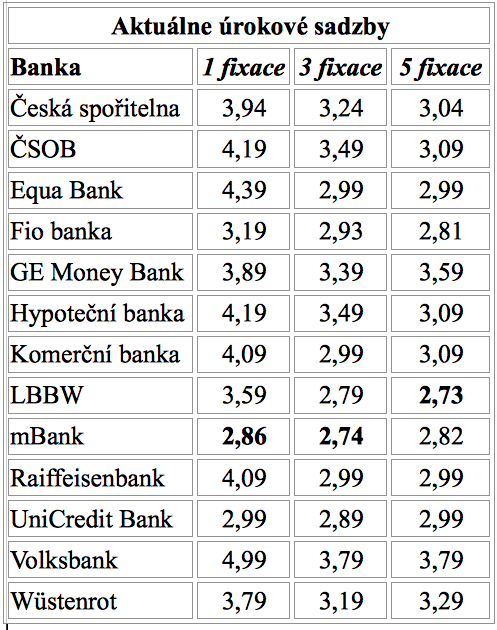
\includegraphics{data/sadzby.png}

\emph{\footnotesize Zdroj:  \href{http://www.hypoindex.cz/zmeny-v-urokovych-sazbach-u-hypotek-petileta-fixace-od-2-73/}
 {http://www.hypoindex.cz/zmeny-v-urokovych-sazbach-u-hypotek-petileta-fixace-od-2-73/} }
 \normalsize

\label{sadzby}
\end{figure}



\end{document}
